\clearpage{\pagestyle{empty}\cleardoublepage}
\chapter*{Introduzione} 
%%\markboth{Introduzione}{Introduzione}
\addcontentsline{toc}{chapter}{Introduzione}
%

%
Secondo il rapporto sullo stato del solare fotovoltaico in Italia
\cite{gse2010}, pubblicato dal \emph{Gestore dei Servizi Energetici}
(GSE) nell'Aprile del 2011, il numero di impianti fotovoltaici
presenti sul territorio nazionale al 31 dicembre 2010 \`e pari 
a 155977, per una potenza nominale complessiva di circa 3469,9 MW.
%
Tali valori si inseriscono all'interno di un trend di crescita, 
mostrato in figura \ref{fotovoltaico-italia}, decisamente sostenuto: 
solo nel 2010, il numero di impianti \`e raddoppiato, mentre la potenza 
nominale \`e addirittura triplicata.
%
Tra le motivazioni alla base di tale crescita, vi \`e sicuramente il 
programma di incentivazione, noto come \emph{Conto Energia}\cite{camera2003},
riservato ai soggetti responsabili di impianti fotovoltaici.
%% %
\begin{figure}[!h]
\centering
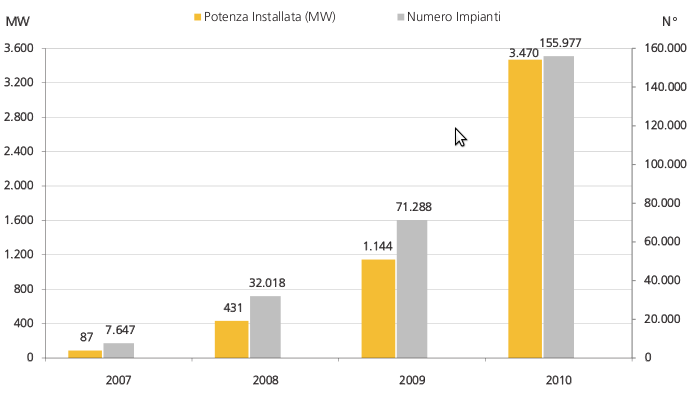
\includegraphics[width=350pt]{img/trend-fotovoltaico-italia.png}
\caption{Trend di crescita del fotovoltaico in Italia}
\label{fotovoltaico-italia}
\end{figure}
%% %
%
\`E interessante osservare che oltre il 90\% degli impianti installati
appartiene alla classe di potenza medio-bassa, i.e. la potenza nominale
non supera i 20kW. 
%
Ci\`o rende l'idea di come la produzione di energia
elettrica mediante fotovoltaico sia fortemente \emph{distribuita} 
sul territorio, in contrasto con i metodi di produzione mediante 
fonti \emph{convenzionali}, ad esempio carbone e gas, che avviene 
in pochi grandi impianti, ciascuno in grado di sviluppare potenze molto 
elevate.
%

%
In un contesto caratterizzato da una crescita vertiginosa e da una 
elevata frammentazione geografica degli impianti, il problema del
\emph{monitoraggio}, inteso come verifica \emph{continuativa} e \emph{remota}
dello stato di un impianto, %% !FIXME che brutta espressione
assume una grande rilevanza: il soggetto responsabile della manutenzione
dell'impianto necessita di uno strumento che gli permetta di
effettuare diagnosi di eventuali malfunzionamenti \emph{da remoto}, cio\'e 
senza intervenire fisicamente sull'impianto; d'altro canto, il soggetto 
responsabile dell'impianto, ovvero il proprietario, \`e interessato 
a verificare se e quanto l'impianto sta producendo, e, quindi, 
tenere sotto controllo il ritorno sull'investimento effettuato.

%% descrizione del contenuto della tesi
